%\thesubsection{Boosted Decision Trees}
\label{app:bdt}
%% As the HLT trigger makes use of a machine learning technique called a Boosted Decision Trees (BDT), an aside will be taken here to introduce the concept.

Many rare decay analyses make extensive use of BDTs and they are important in the \Lbpi analysis. Firstly, the concept of a decision tree is introduced followed by a brief explanation of boosted decision trees.

A decision tree, in the context of data mining, is a supervised machine learning method which allows for the prediction of the value of a target variable based on several input variables. In particle physics, the purpose of the decision tree is to classify an event as being either signal or background, based on the event's input variables. The input variables, $\left\{x_{i}\right\}$, are various physics parameters. % and in the case of the HLT include the minimum $P_{T}$  and mass of the particle.
% and $IP_{\chi2}$ (where the $IP_{\chi2}$ is the difference in the $\chi2$ of the fit to the PV when the track whose $IP_{\chi2}$ is being measured is added and then removed)
Each cut point in the tree is referred to as a node and the final nodes are referred to as leaves. A very simple example is shown in~\autoref{fig:BDT}. The purity, $P$, of a leaf refers to the fraction of the weight of a leaf due to signal events, e.g. if a leaf had 20 signal events and 15 background events it would have a purity of 0.75. If a leaf has a purity larger than 0.5 it is deemed to correspond to signal and if lower, to background.
\begin{figure}
  \centering
  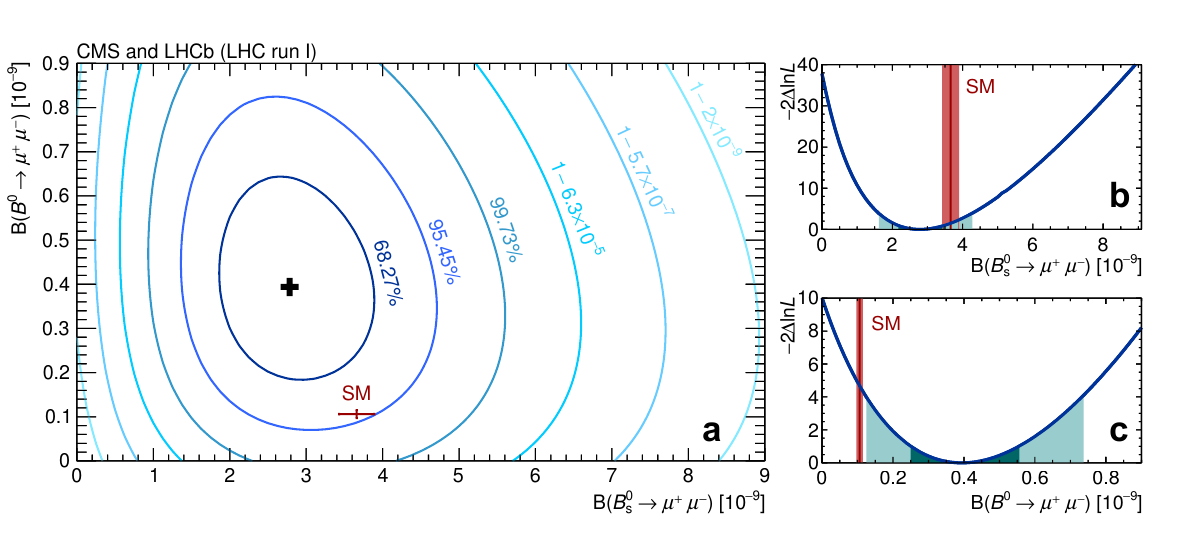
\includegraphics[scale = 0.7]{figs/BDT.png}
  \caption{An example decision tree. The S and B stand for `Signal-like' and `Background-like'. The $\beta_{i}$ variables refer to the cut values chosen by the machine learning algorithm after the tree has been trained on signal and background samples. The blue ovals represent final nodes called leafs, which each leaf having an associated purity, i.e. the fraction of the weight of a leaf due to signal events.}
  \label{fig:BDT}
\end{figure}

A decision tree is constructed by a process called training. For this, samples of known signal and background events are used. These samples could be either simulation or data. For each $x_{i}$ the best dividing point is decided, that is, the cut that gives the best separation between signal and background. This optimum point is decided by using the Gini index defined as

\begin{equation}
Gini  = \sum^{n}_{i = 1} W_{i} P(1 - P),
\end{equation}
where $W_{i}$ is weight of the $i^{th}$ event, which would generally be unity for the case of a non-boosted decision tree. 
The cutting point is then found by maximising the separation, $\Delta$, between the Gini index of the parent node and the combined Gini index of the child nodes, as given in~\autoref{eq:diffgini} 
\begin{equation}
 \Delta =   Gini_{parent} - Gini_{child_{1}} - Gini_{child_{2}}.
  \label{eq:diffgini}
\end{equation}
The depth of a tree (the maximum number of cuts or nodes) is normally a number specified before the training begins.
%\cite{miniboone}

Boosting a decision tree involves training many trees ($\mathcal{O} \sim 1000$) and giving misclassified events a higher weight. A misclassified event is defined as a known signal event being placed on a background leaf and vice versa. By giving the events which are difficult to classify more weight, the next tree to be trained will effectively have to work harder in order to classify events correctly. %The way in which events are weighted (or boosted) can vary, and in the 

The total score on an event is deduced by following an event through from tree to tree and, for the algorithms used in this thesis, is simply given by the weighted sum of the scores over the individual trees.

%% This weighting is done using the total number of misclassified events in a tree. The error of the $m^{th}$ tree is defined as
%% \begin{equation}
%%   err_{m}=\sum_{j}W_{j}; j = \text{misclassified event}.
%% \end{equation}
%% The weight (or score) of this tree is then given as
%% \begin{equation}
%%   \alpha_{m} = C \ln\frac{1-err_{m}}{err_{m}},
%% \end{equation}
%% where $C$ is  a constant. The increase in weight of a misclassified event is given as
%% \begin{equation}
%%   W_{i} = W_{i} e^{\alpha_{m}}.
%% \end{equation}
%% All weights are then renormalized, $W_{i} \to W_{i}/\sum^{N}_{i = 1} W_{i} $, and the total output, $T(x_{i})$, for an event $i$ is given as
%% \begin{equation}
%%   T(x_{i}) = \sum^{N_{tree}}_{m = 1} \alpha_{m}T_{m}(x_{i}).
%% \end{equation}

Data sets are split into two (or more) sub samples, where one half is used for training the tree and the other is used for testing the tree, and the distributions of the event scores (the BDT output) for training and testing samples are compared for signal and background. Cases where the training sample performs better than the testing sample are referred to as over-trained trees, which is often due to the BDT becoming sensitive to the statistical fluctuations of the training sample.%Most BDT's used within LHCb produce a BDT output ranging from -1 to 1, with more positive outputs being associated with a more signal-like data candidate.

 The distribution of events scores for a given dataset can then be cut on in order to increase the fraction of signal events.

%Alternatively, the over performance of the training sample could be due to there being correlations between the  signal and background proxies used for training which do not exist in the actual data. 
%% The value for $G$ is calcualted using the Gini index which is a function of the purity $p$.


%% The creates two new nodes and the algorithum is applied again to these nodes. Adapative boosting is when misclassfied events (i.e. in the case when you have a signal training sample the event is classified as abckground and vice versa) and given higher weighs 
%% For each xi the splitting value that gives the best separation of the events into two child nodes -- one with mostly signal events, the other with mostly background events -- is found. The variable and split value giving the best separation are selected and two new nodes are created, one corresponding to events satisfying the split criterion (labeled P for passed in the above figure), the other containing events that failed it (labeled F). The algorithm is then applied recursively to the two child nodes. This process contains untill the specified maximum number of given nodes. When the splitting stops, the terminal node is called a leaf, with an associated purity, the weighted signal fraction of the training sample in this node

%The primary vertex is defined as being within a raduis of 300\mum of the mean position of the $pp$ interation. 


